% Template taken from https://www.sharelatex.com/templates/journals/template-for-the-journal-of-machine-learning-research-jmlr

\documentclass[twoside,11pt]{article}

% Any additional packages needed should be included after jmlr2e.
% Note that jmlr2e.sty includes epsfig, amssymb, natbib and graphicx,
% and defines many common macros, such as 'proof' and 'example'.
%
% It also sets the bibliographystyle to plainnat; for more information on
% natbib citation styles, see the natbib documentation, a copy of which
% is archived at http://www.jmlr.org/format/natbib.pdf

\usepackage{jmlr2e}
\usepackage{amsmath}
% Definitions of handy macros can go here

\newcommand{\dataset}{{\cal D}}
\newcommand{\fracpartial}[2]{\frac{\partial #1}{\partial  #2}}

% Heading arguments are {volume}{year}{pages}{submitted}{published}{author-full-names}

\jmlrheading{1}{2019}{1-10}{9/19}{9/19}{George Engel, Troy Oster, Dana Parker, Henry Soule}

% Short headings should be running head and authors last names

\ShortHeadings{CSCI 447: Project 1}{Engel, Oster, Parker, Soule}
\firstpageno{1}

\begin{document}

\title{CSCI 447: Project 1}

\author{\name George Engel \email GeoEngel.z@gmail.com \\
       \addr Department of Engineering\\
       Montana State University\\
       Bozemane, MT 59715, USA
       \AND
       \name Troy Oster \email toster1011@gmail.com \\
       \addr Department of Engineering\\
       Montana State University\\
       Bozeman, MT 59715, USA
       \AND
       \name Dana Parker \email danaharmonparker@gmail.com \\
       \addr Department of Engineering\\
       Montana State University\\
       Bozeman, MT 59715, USA
       \AND
       \name Henry Soule \email hsoule427@gmail.com \\
       \addr Department of Engineering\\
       Montana State University\\
       Bozeman, MT 59715, USA}

\editor{Engel et al.}

\maketitle

\begin{abstract}%   <- trailing '%' for backward compatibility of .sty file

In this assignment, we implemented the naive Bayes machine learning algorithm [3] on 5 data sets. We utilized 10-fold cross-validation to test our implementation and measured difference in accuracy between the average accuracy returned by the cross-validation of the original data set and the average accuracy returned by the cross-validation of the data set with 10\% noise applied, using two loss functions: 0-1 Loss, and Precision/Recall [1]. 

\end{abstract}

\begin{keywords}
    naive Bayes, 0-1 Loss, Precision/Recall, cross-validation, 
%   Bayesian Networks, Mixture Models, Chow-Liu Trees
\end{keywords}

\section{Introduction}
The naive Bayes classification model [3] is a simple model for predicting data classification. In this assignment, we implemented this probabilistic model on multiple real-world data sets. We validated our implementation of the algorithm with 10-fold cross-validation and measured the performance of our implementation with two loss functions: 0-1 Loss, and Precision/Recall.

\section{Problem Statement}
Given a data set of which all the correct classifications are known, we can implement and execute a training algorithm on a subset of the data. Then, once trained, the algorithm will guess the classes of another subset of the data and measure the performance. For this assignment, we were provided with 5 real-world data sets. Our task was to implement a training algorithm and guess classifications for each of these 5 data sets and then utilize two different loss functions to measure the accuracy and performance of our predictions. We ran this algorithm on the original versions of each data set, and then introduced noise to each of the data sets by shuffling attribute values among 10\% of the values, and ran the algorithm of the five shuffled versions of the data. So now we want to know how the noise introduced via shuffling will affect our accuracy. \\
\section{Hypotheses}

\subsection{Breast Cancer Wisconsin} This data set is comprised of 9 quantitative variables, and each data example can be classified as either benign or malignant. We hypothesized that, given that there are only two possible classifications, that we will achieve no less than 85\% accuracy (i.e. a 0-1 Loss score of 0.75) on our un-shuffled data. We think that the shuffled breast cancer data will be no more than 3\% less accurate.
\subsection{Glass} This data set is comprised of 7 quantitative variables, and each data example can be classified as one of 7 possible glass types: building\_windows\_float\_processed, building\_windows\_non\_float\_processed, vehicle\_windows\_float\_processed, vehicle\_windows\_non- \\ \_float\_processed, containers, tableware, or headlamps. We hypothesize that we will achieve no less that 65\% accuracy (0-1 Loss of 0.65) for the un-shuffled data, given that there are 7 potential classes. The shuffled data, we predict, will be no more than 5\% less accurate than the shuffled data.
\subsection{Iris} This data set is comprised of 4 quantitative variables. Each data example can be classified as one of three different flower types. We are predicting approximately 75\% (0-1 Loss of 0.75) accuracy.
\subsection{Soybean} This data set is comprised of 35 attributes, and each data example can be classified as one of four different classifiers. We hypothesize 70\% accuracy (0-1 Loss of 0.7) for this un-shuffled data. For the shuffled data we are predicting the accuracy to be approximately 3\% less accurate.
\subsection{Voting Records} This data set is comprised 16 categorical attributes, and each example may be classified as either republican or democrat. We are hypothesizing approximately 85\% accuracy (0-1 Loss of 0.85) for this dataset. We are predicting that the shuffled voting-record data should no more than 3\% less accurate than the shuffled data.\\

\section{The Algorithm}
Per the instructions of the assignment, we implemented the naive Bayes algorithm on the 5 provided data sets. Given some example $x \in X$, where $X$ is our data set, naive Bayes predicts the correct class $c$ of $x$ by computing the probabilities of each possible classification for $x$. For class $c$, the probability is denoted as $P(c | a_1, a_2,...,a_d)$ where $a_k$ denotes one of $d$ attribute values in $x$. To compute this probability for each class $c$, the probabilities of each attribute value are computed. For each attribute value $a_k$, we compute $P(c) * \prod^d_{i=0} P(a_i | c)$, where $P(c)$ is the probability of an attribute being classified as class $c$. To predict the correct class for $x$ we compute $\underset{c \in C}{\mathrm{argmax}}$ $P(c) * \prod^d_{i=0} P(a_i | c)$.

\section{Our Approach}
\subsection{Handling missing data}
 We opted to not remove data with missing values that occurs in low quantities, as given the already-small size of the data sets we are working with for this assignment, we thought it best to retain as much data as possible for training purposes.

Rather, we decided to handle missing attribute values by replacing them with attributes selected randomly from a bootstrap distribution generated from all other data points in the database of the same attribute type that do not contain missing values. 

It is also worth noting that we do not hard code the symbol used for checking for missing values, but rather the missing value symbol is determined in the configuration '.attr' file that is unique for each database. It was handled in this manner due to inconsistencies between data sets with respect to symbols representing missing data.

\subsection{Handling information about Attributes}
Due to the fact that the databases had some uniqueness about them, rather than changing them directly to fit a generic format, we found it best to add a short and sweet configuration file for each database that would determine certain values when running our code. This way, we can both easily customize our parameters, and not have to rely on something primitive like command line user input. 

The configuration file being referred to is the '.attr' file that exists in the directory of each database. it is required that the respective attribute configuration file ('.attr' file) has the same prefix as the '.data' file for the database in order to function, as our code base looks for the '.data' file in the database directory specified, and then uses the prefix of the file name when locating the attribute file. 

The attribute file contains things like the column headers, column index of the attribute we want to classify, a list of indexes of the parameters used for classification, and finally, the last line is what will be used as the 'missing symbol', which is referenced in section (4.1). When running the program, these values are loaded in after the user selects a database from the list presented, and used accordingly.

\subsection{Separating and classifying data}
To properly implement naive Bayes [3] on the 5 data sets, we first needed to properly separate and classify each data set. Each data set needed to be separated by class, and then the count and probability of each attribute value for each class needed to be computed. Our approach for this was to create, for each dataset, an associative array, where each possible classifier was a key. For each key, the corresponding values were each their own associative arrays, the keys of which were all the extant attribute values among that class. The value of each key in these inner arrays was a set storing the count and conditional probability of each attribute value given the respective class. \\ \\

\subsection{K-Fold Cross Validation}
We tested our algorithm's implementation using 10-fold cross-validation. This validation model separates each data set into 10 subsets, or "bins", of equal size. It then runs 10 iterations. During each iteration, one bin is designated as the test data, being the data we will test our prediction algorithm on. The other 9 bins are designated as training data. It is on this training data subset that we will execute our learning algorithm, from which we will base our predictions. After first running the training algorithm on these 9 bins, we then predict the classifications of each example in the designated test data. For each iteration, a different bin is designated as test data, while the other 9 are designated as the training data. \\ \\

\subsection{Shuffling/Applying Noise}

In addition to implementing our prediction algorithm for the plain version of each data set, we also ran it with a 10\% noise modifier applied to the training data set in order to try and grasp how noise might affect the naive bayes machine learning algorithm. 

We implemented our prediction algorithm on the original version of each data set, and also introduced noise to each data set by randomly selecting 10\% of each data set and the shuffling attribute values. We then ran our algorithm on these shuffled versions of each data set.

\subsection{Loss functions}
To assess the performance of our class prediction algorithm, we implemented two loss functions: Precision/Recall, and 0-1 Loss. We ran both loss functions on each iteration of the 10-fold cross-validation process, and then took averages of the values returned during from each iteration and used these values to measure the performance of our prediction algorithm. 0-1 Loss simply computes the fraction of the data our algorithm correctly classified. For each correctly classified data example, a 0 is returned, and for every incorrectly classified value, a 1 is returned. Accuracy is then defined as the percentage of 0's returned [2].\\ \\

\subsection{Loss function 1: Precision Recall}
The Precision/Recall loss function computes two values, known as precision and recall, to measure the performance of our class prediction algorithm. This loss function utilizes the amounts of true positive, false positive, and false negative classifications for each class. Precision and recall are are computed as follows: 
$$Precision = \frac{1}{|C|} \sum^{|C|}_{i=1} \frac{TP_i}{TP_i + FP_i}$$
$$Recall = \frac{1}{|C|} \sum^{|C|}_{i=1} \frac{TP_i}{TP_i + FN_i}$$
$TP_i$ denotes the number of true positive classifications for class $i$, $FP_i$ denotes the number of false positive classifications for class $i$, and $FN_i$ denotes the number of false negative classifications for class $i$. $C$ is the set of all possible classes. Precision can be interpreted as a measure of how accurate true positive classifications are, as it computes the fraction of all positive classifications for a class that were truly positive. Recall measures accuracy among the values for each class that should have been positive, as it computes the fraction of all values that truly belonged to a class that were classified as positive [1]. \\ \\


\section{Results}
\begin{figure}[!hbp] % Credit to stack exchange user Masroor and user Stefan Kottwitz for the implementation of side by side figures in LaTeX
    \centering
    \begin{minipage}[b]{0.7\textwidth}
      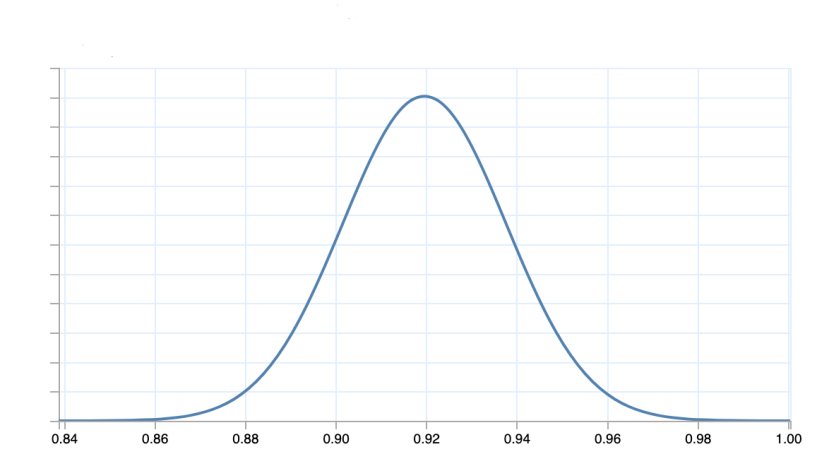
\includegraphics[width=\textwidth]{01_loss_graph.png}
      \caption{Average 0/1 Loss for \emph{Iris} (over 1,000 iterations)}
    \end{minipage}
    \hfill
    \begin{minipage}[b]{0.4\textwidth}
      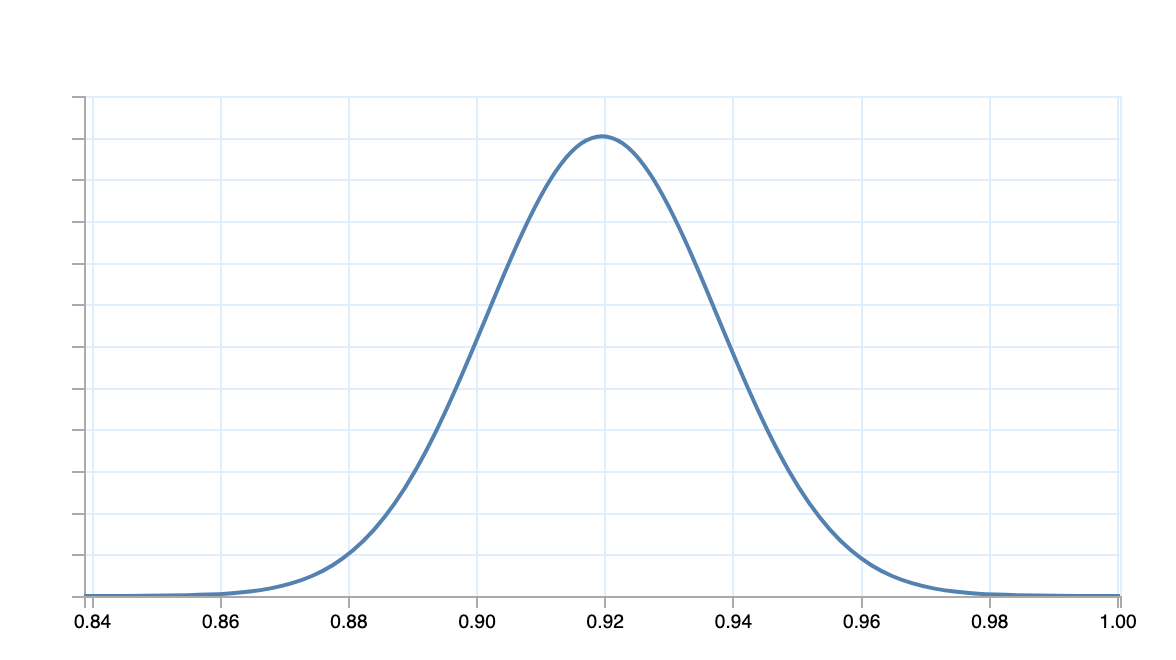
\includegraphics[width=\textwidth]{precision_graph.png}
      \caption{Average Precision for \emph{Iris} (over 1,000 iterations)}
    \end{minipage}
    \hfill
    \begin{minipage}[b]{0.4\textwidth}
        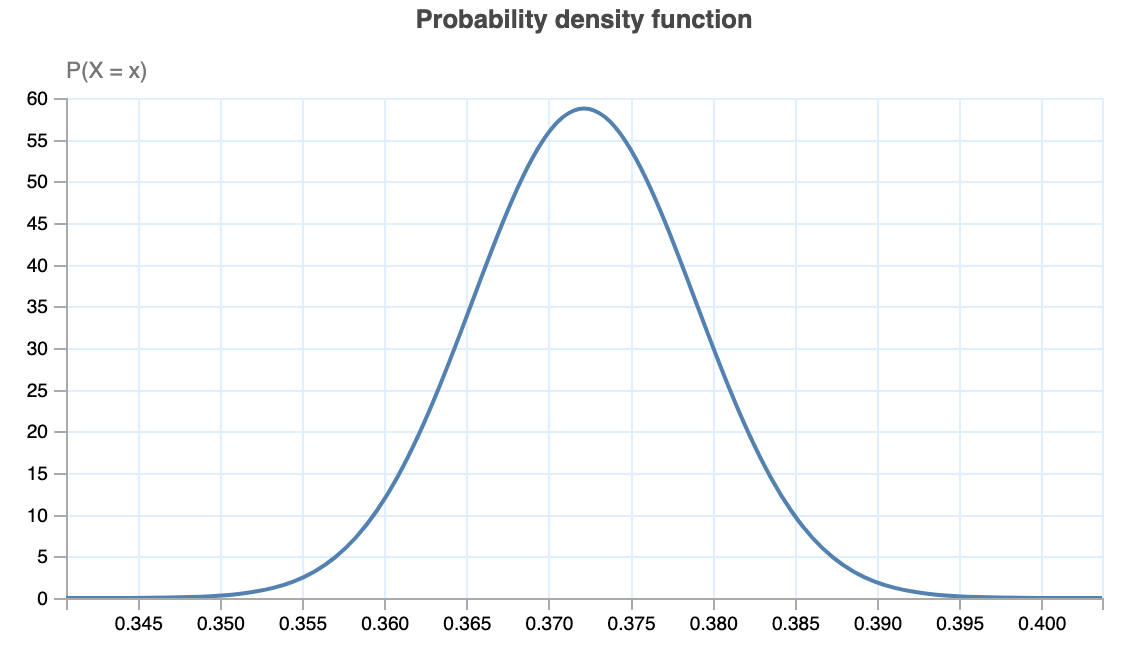
\includegraphics[width=\textwidth]{recall_graph.png}
        \caption{Average Recall for \emph{Iris} (over 1,000 iterations)}
    \end{minipage}
\end{figure}

The graphs shown are of the normal distribution of the values obtains from our loss functions for the iris data set, with 10\% noise applied. 

To construct these graphs, we ran 1,000 iterations of 10-fold cross-validation and found the average for the 0-1 Loss, precision, and recall against the Iris database. For the graph relating to Iris' recall over 1,000 iterations of 10-fold cross-validation, we are 95\% confident that the true recall for our naive Bayes algorithm's ability to classify test data is between 0.359 and 0.386 via a 95\% confidence interval. Regarding 0-1 Loss (the proportion of correct guesses by the naive Bayes algorithm), we are 95\% confident that the true 0-1 Loss for our naive Bayes algorithm's ability to classify test data is between 0.884 and 0.956 via a 95\% confidence interval. Finally, regarding precision, we are 95\% confident that the true precision for our naive Bayes algorithm's ability to classify test data is between 0.394 and 0.405 via a 95\% confidence interval.

% Acknowledgements should go at the end, before appendices and references

\acks{1. Davis, Jesse, and Mark Goadrich. "The Relationship between Precision-Recall and ROC Curves." Proceedings of the 23rd International Conference on Machine Learning - ICML 06, 2006, doi:10.1145/1143844.1143874. \\ \\
2. Dietterich, Thomas G. "Machine Learning for Sequential Data: A Review." Lecture Notes in Computer Science Structural, Syntactic, and Statistical Pattern Recognition, 2002, pp. 15-30., doi:10.1007/3-540-70659-32. \\ \\
3. Nédellec, Claire, and Céline Rouveirol, editors. “Machine Learning: ECML-98.” Lecture Notes in Computer Science, Springer Berlin Heidelberg, 1998. pp. 1-2., doi:10.1007/bfb0026664.}

\end{document}